%% ----------------------------------------------------------------------------
% BIWI SA/MA thesis template
%
% Created 09/29/2006 by Andreas Ess
% Extended 13/02/2009 by Jan Lesniak - jlesniak@vision.ee.ethz.ch
%% ----------------------------------------------------------------------------
\newpage
\chapter{Experiments and Results}
\label{ch:experimentsandresults}
In this chapter several experiments are implemented for different network designs and input sources, presenting accuracy results on test data. In the context of deep learning a study of those variations on the investigated task is often referred as an ablation analysis. The ordering network analyzed in this thesis is split up in a backbone network and a processing network, to eventually allow for transfer learning although this is not attempted in this work. Instead various feature maps, combinations and some additional experiments are studied, with a discussion about the semantic understanding following in Chapter \ref{ch:discussion}.

For all experiments an stochastic gradient descent method with a momentum of 0.9 was used, employing L2 regularization with a weight decay of 0.001. The base learning rate has been set to 0.01 with a multistep policy to decrease the learning rate by a factor 10 at the 2000, 5000 and 8000 epochs. Training was done for a total of 10000 epochs with a batch size of 16, longer iterations have not shown any significant improvements. It is stressed that finding the precise optimal value of these before mentioned parameters is not the focus of this work and therefore not done separately for all the network variations, but the values have been manually tuned for good general behavior in training. Enforcing the same values for all the different experiments made it easier to compare the results. Networks took up to around 24 hours to complete training, but it should be noted that no early stopping was enforced and most networks did not see significant improvements after approximately 6-12 hours of training.

\section{Feature maps}
A simpler version of the proposed OPN network~\cite{lee2017} has been implemented first, referred with OPN3 from now on. Here the studied permutation task was reduced to the binary ordering task and also the number of input images has been set to 3, to basically have a simple 3-way tuple task as suggested by ~\cite{misra2016} however employing the pairwise feature extraction layers and better initialization parameters for the underlying Caffenet~\cite{jia2014}. Running the suggested network from~\cite{misra2016} without those improvements was also attempted, but poor convergence has been observed. 

This OPN3 network was used with a Caffenet backbone on both the grayscale images generated with the channel splitting, color and unprocessed lidar data (from the direct projection). The results are shown in the upper part of Table \ref{tab:indiv_results}. It is immediately clear that the networks performs remarkably well on the binary classification task, with percentages above 75\% on all different training variations. This is significantly higher than the 50\% which would result from random choice and seems relatively high given the apparent complexity of the task. 

%More details on how this high percentage is reached will be studied in Chapter \ref{ch:discussion}, where an in-depth analysis of the features the network learns is presented, to try to develop a deeper understanding of the network. 

%In general it can be concluded that all the studied OPN3 networks exhibit significant over-fitting, with accuracies reaching close to 100\% on the training data with proper L2 regularization employed. Despite the overfitting, accuracy percentages remain high on the test task a feature seen more often in neural networks. In any case, it becomes clear that the binary ordering task can be relatively easy for the neural network to learn, as was noticed earlier by Fernando et al.~\cite{fernando2017}.
%Despite the overfitting, accuracy percentages remain high on the test task a feature seen more often in neural networks.
From this it follows that the the binary ordering task is relatively easy, as was noticed earlier by Fernando et al.~\cite{fernando2017}. All the studied OPN3 networks also exhibit significant over-fitting, with accuracies reaching very close to 100\% on the training data and test data with proper L2 regularization employed. Therefore all successful experiments on the OPN3 have also been carried out on the full OPN network\cite{lee2017}, with 4 images as input and permutation labeling. In contrast to the OPN network presented in the paper, which does not distinguish between forward and backward orderings of the same permutation, in this work the network are trained with all 24 permutation labels treated distinct, as it is expected that in driving videos the difference between going forward (as would happen in reality) and going backward should be detectable. The variation used in this work is referred as OPN4 in the rest of this thesis.

Again the remainder of Table \ref{tab:indiv_results} show also strong performance of the OPN4 network, despite the supposed complexity. With a fully random network gaining an accuracy of around 4\%, the version using only grayscale already shows a very significant improvement with over 51\% accuracy. On the OPN3 network it is observed that both the version on grayscale and color images work better than the unprocessed lidar which could be expected because the image generally provides a richer representation of the world with more attention to details. This behavior is also seen in the full OPN4 network with the grayscale and color images showing significantly higher accuracies compared to the unprocessed lidar. Moreover the grayscale version performs slightly better then the color in the OPN4 network, confirming that extra regularization in the form of channel splitting helps in preventing overfitting and thus increases the overall quality of the learned features, although this effect is not seen on the OPN3 network (possibly because the difference is negligible and that the difference fits in the training uncertainty).

%supposedly because it contains enough information to develop and understanding of the world and the channel-splitting also serves as a protection against overfitting. Just like in the OPN3 network the unprocessed lidar depth is less strong than both the color and grayscale versions.

%In comparison to the OPN3 network it is speculated this is the result of the channel splitting producing too strong modifications which work good agains the overfitting in OPN3, but the complexity of the task itself already produces enough guidance in OPN4 for the network to learn better features. 

Besides the unprocessed lidar depth from the direct projection investigated with the OPN3 network, also other data generated from the lidar is examined but only with the OPN4 network. First a CNN is trained using the lidar reflectances, which feature maps could be seen as a poor man's version of a camera. This network does surprisingly not converge at all, with accuracy sticking around 4\%, from which it follows that the added detail in grayscale and color images leads to a significant improvement compared to the reflectances captured by lidars. Secondly, a network with the height above ground was investigated reaching a percentage around 35\%, higher than the unprocessed lidar depth, which might be expected to be a stronger feature. It is however interesting to note that the height above ground functions as a feature invariant to movement, as the height of for example a certain car remains the same in different frames independent of the movement of the particular car. Nevertheless, it becomes evident that the depth is still a strong feature, and it becomes much stronger after applying a interpolation strategy with an accuracy very strong performance close to 60\%. In theory the neural network should be able to learn this conversions from a sparse map itself, but it is evident that additional preprocessing benefits the learning significantly. Unfortunately this suggested interpolation strategy does not naturally extends to the height above ground as this height is expected to change linearly over common approximately box-like objects like cars instead of mostly being constant. 

%The generation of these additional features is based on the HHA encoding\cite{gupta2013}, with the horizontal disparity map generated using interpolation of the unprocessed depth map and a height map by estimating the direction of gravity and calculating the distance above the lowest point (the measured angle is not investigated). Both those features show improved performance, with the interpolated depth in particular showing very strong performance close to 60\% accuracy, from which it can be concluded that the learning can benefit substantially from using interpolated version. It is also surprising to see that the estimated height shows relative strong performance, in particular compared to the unprocessed lidar depth. Finally the reflectances are apparently to weak source of information for the network to converge.

%%% ADD SOME REAOSING ABOUT THE LIDAR HEIGHT (AND DEPTH) HERE

\begin{table}[]
\centering
\caption{Accuracy results for the sorting task on different individual features (italic indicates non-converging)}
\label{tab:indiv_results}
\begin{tabular}{|p{7.5cm}|p{2cm}|p{2cm}|}
\hline
\textbf{Input}                                                          & \textbf{Output network} & \textit{\textbf{Accuracy}} \\ \hline
grayscale                                                               & OPN3                    & 82.3 \%                   \\ \hline
color                                                                   & OPN3                    & 84.3 \%                   \\ \hline
unprocessed lidar depth                                                 & OPN3                    & 75.9 \%                   \\ \hline
grayscale                                                               & OPN4                    & 51.2 \%                   \\ \hline
color                                                                   & OPN4                    & 44.5 \%                   \\ \hline
unprocessed lidar depth                                                 & OPN4                    & 27.3 \%                   \\ \hline
unprocessed lidar reflectances                                          & OPN4                    & \textit{4.8} \%                   \\ \hline
lidar height                                                            & OPN4                    & 35.2 \%                   \\ \hline
interpolated lidar depth                                                & OPN4                    & 59.3 \%                   \\ \hline
\end{tabular}
\end{table}

\begin{figure}[t!]
\centering
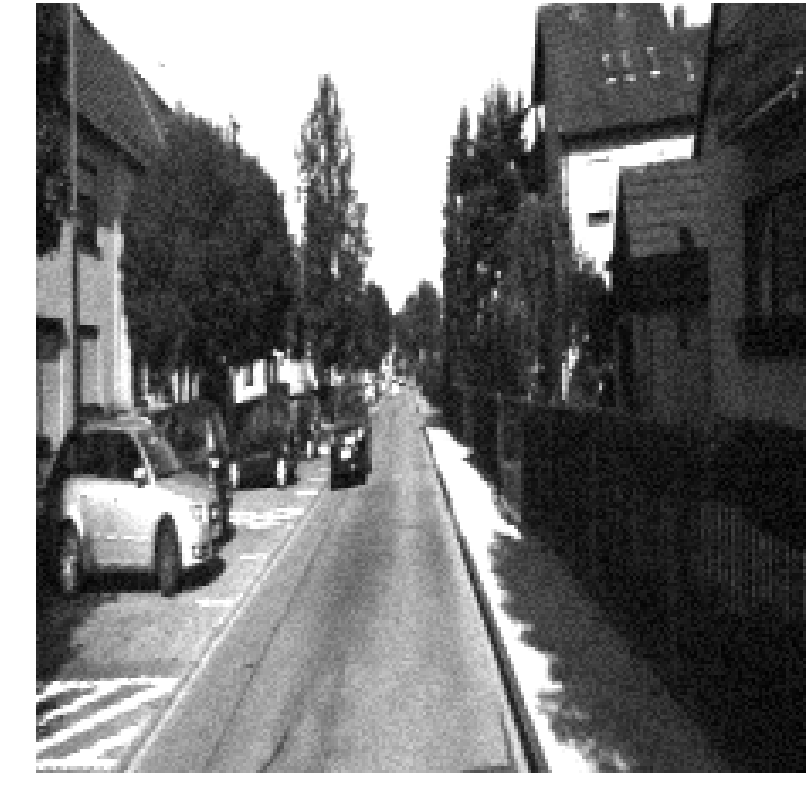
\includegraphics[width=0.32\textwidth]{images/gray_image1.png}
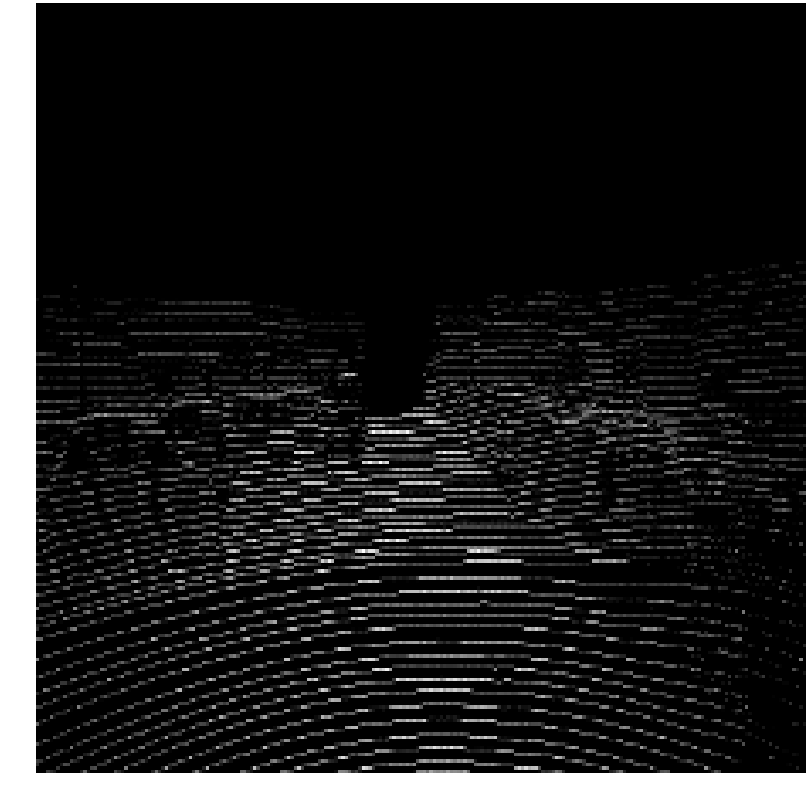
\includegraphics[width=0.32\textwidth]{images/height_image1.png}
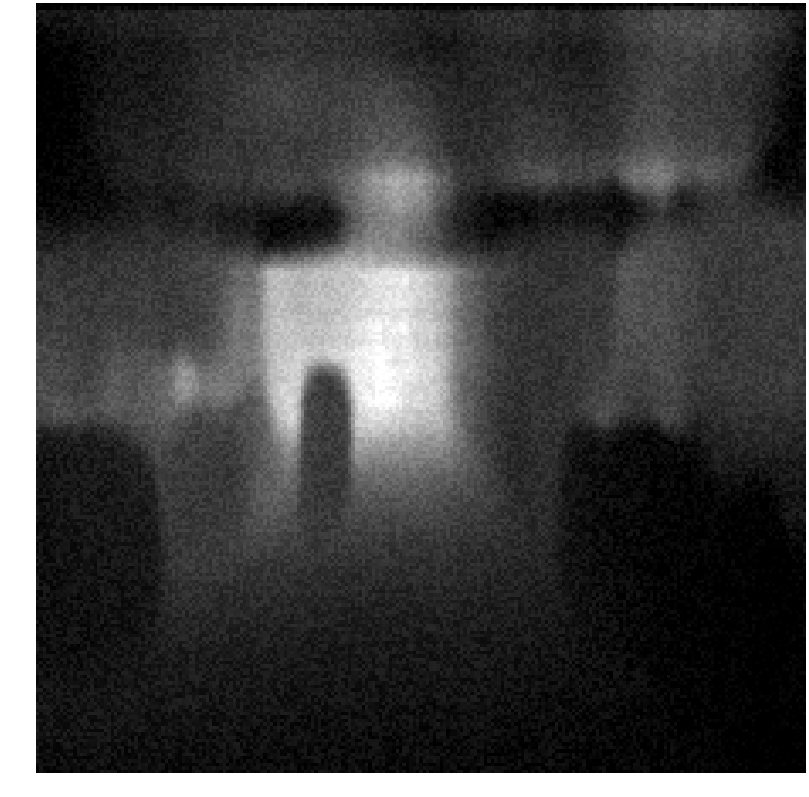
\includegraphics[width=0.32\textwidth]{images/depth_image1.png}
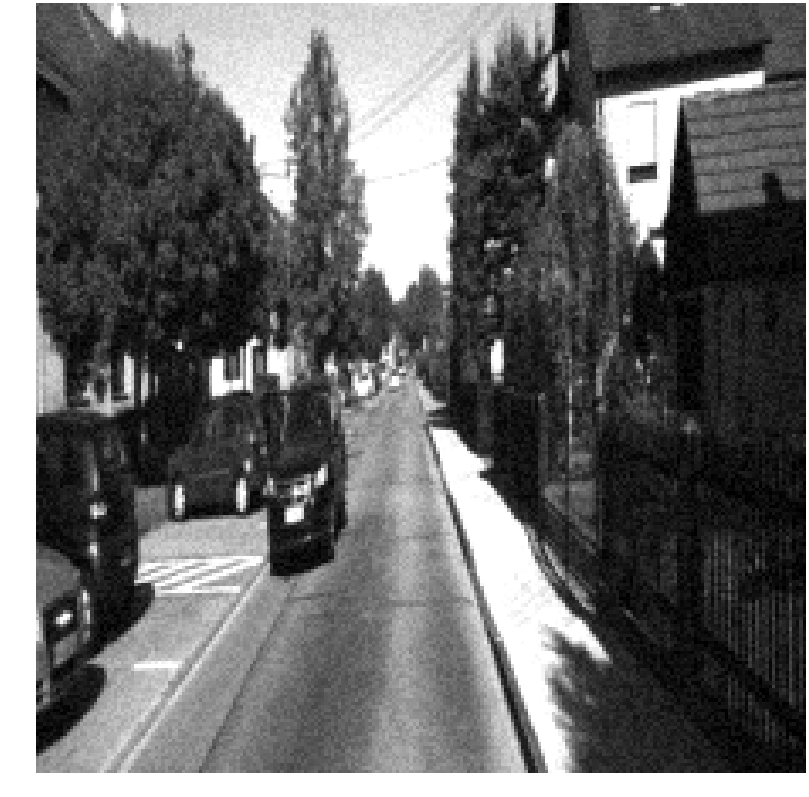
\includegraphics[width=0.32\textwidth]{images/gray_image2.png}
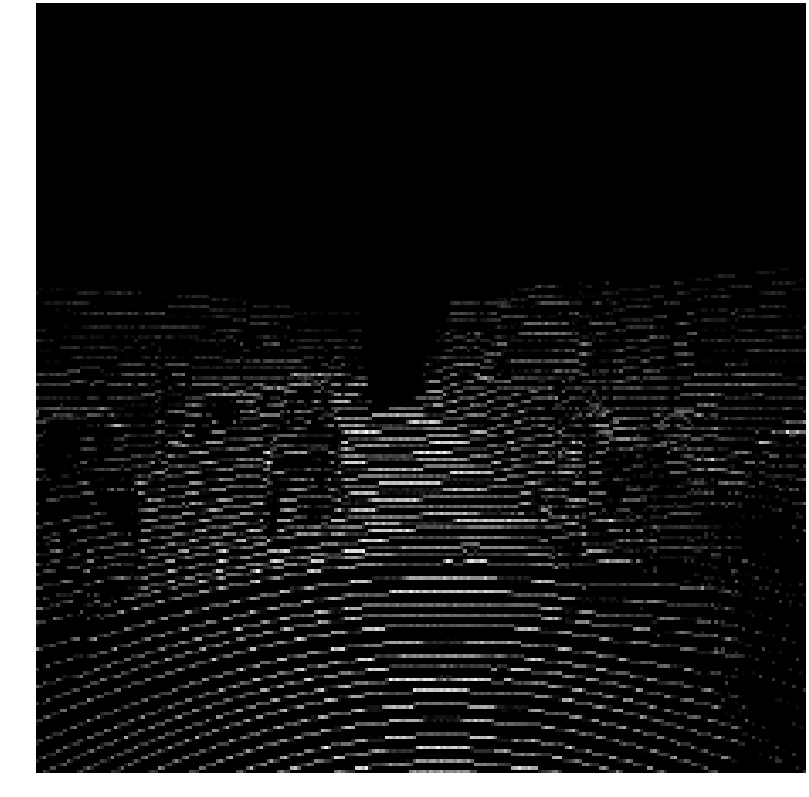
\includegraphics[width=0.32\textwidth]{images/height_image2.png}
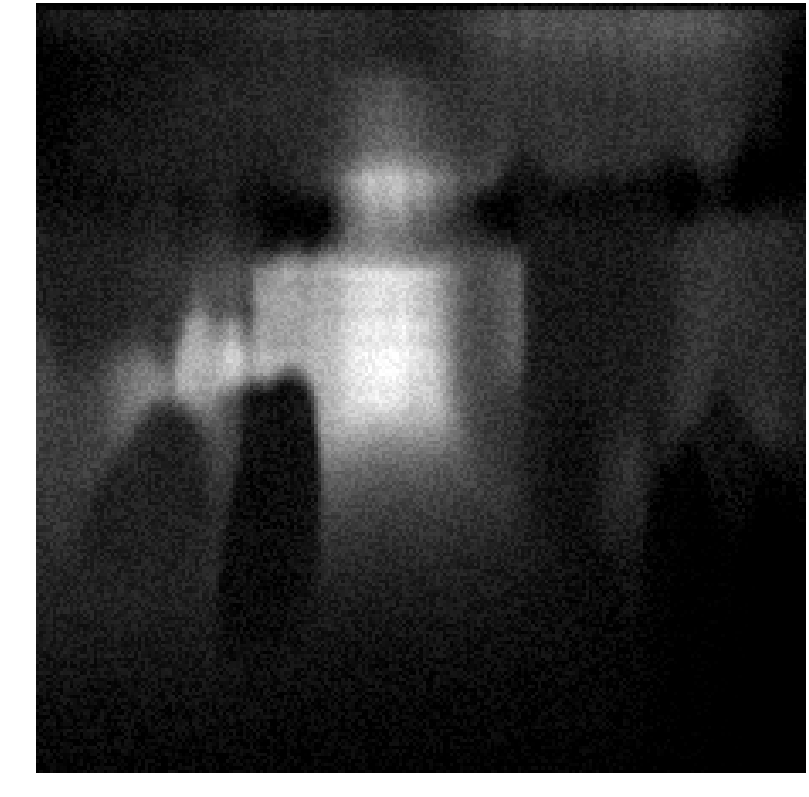
\includegraphics[width=0.32\textwidth]{images/depth_image2.png}
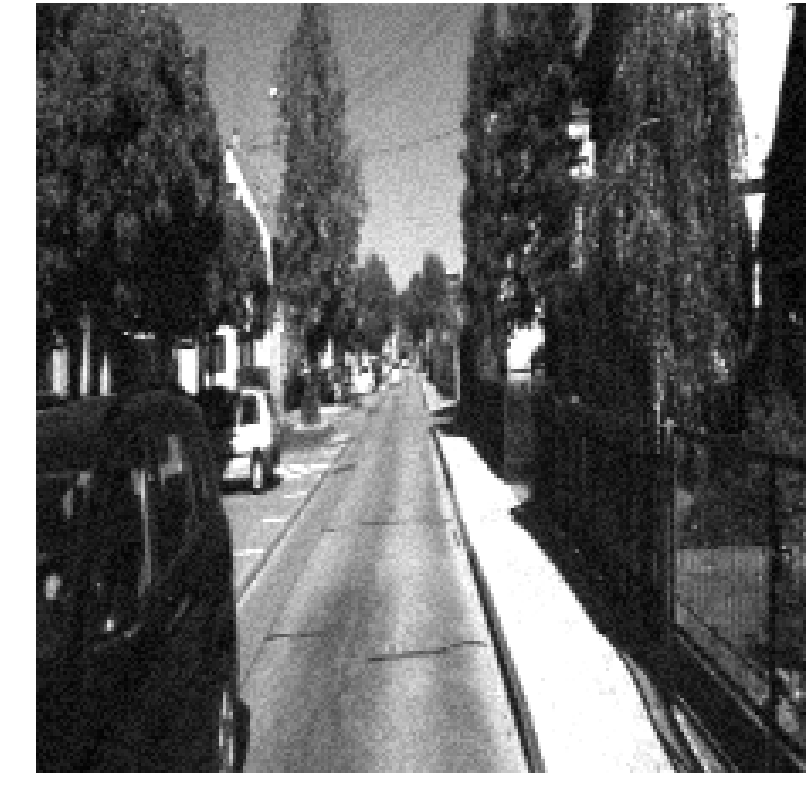
\includegraphics[width=0.32\textwidth]{images/gray_image3.png}
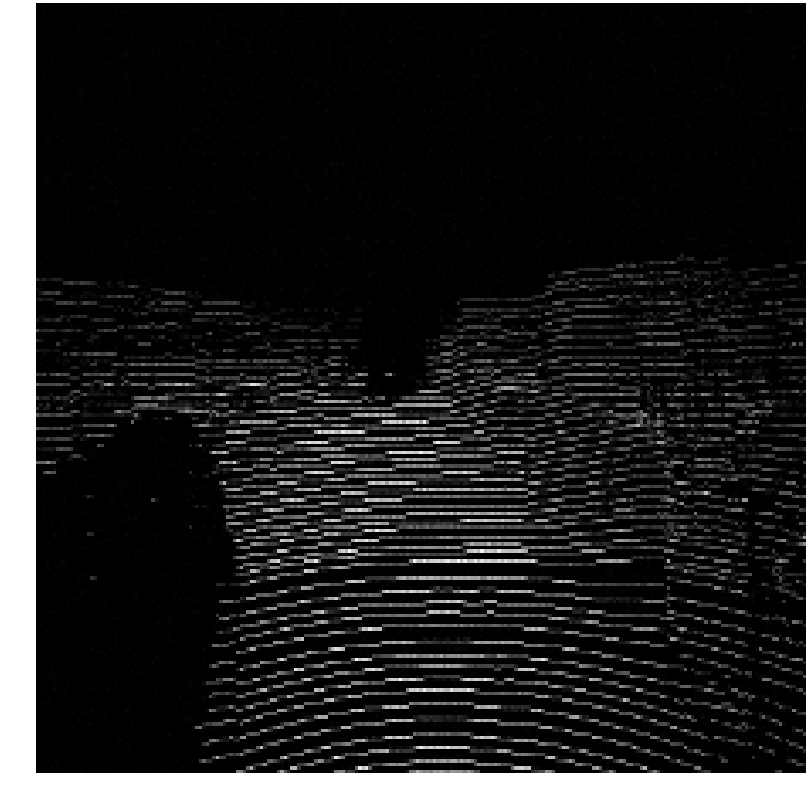
\includegraphics[width=0.32\textwidth]{images/height_image3.png}
\fcolorbox{red}{white}{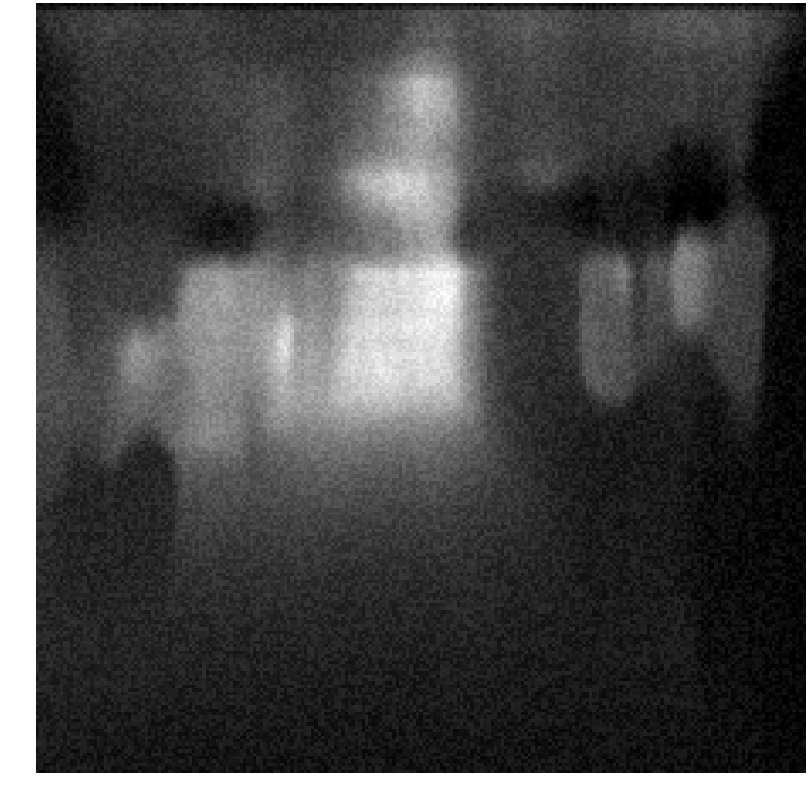
\includegraphics[width=0.32\textwidth]{images/depth_image4.png}}
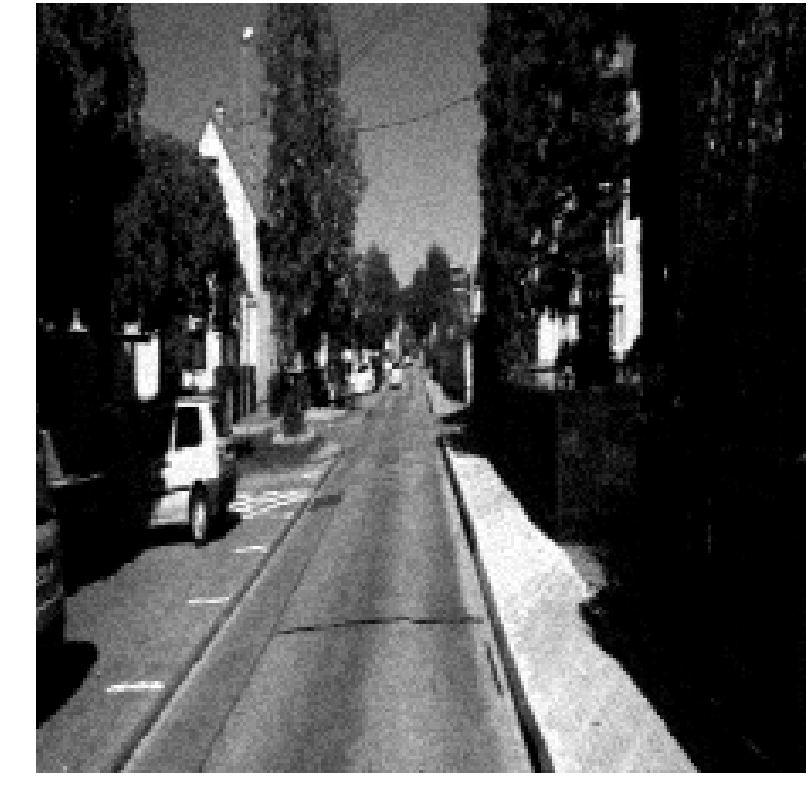
\includegraphics[width=0.32\textwidth]{images/gray_image4.png}
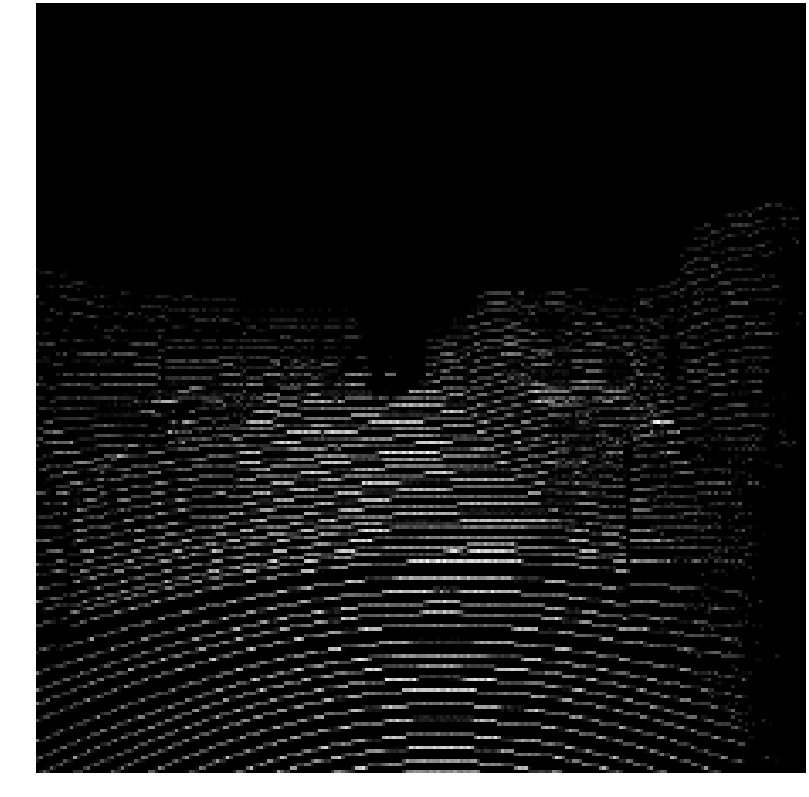
\includegraphics[width=0.32\textwidth]{images/height_image4.png}
\fcolorbox{red}{white}{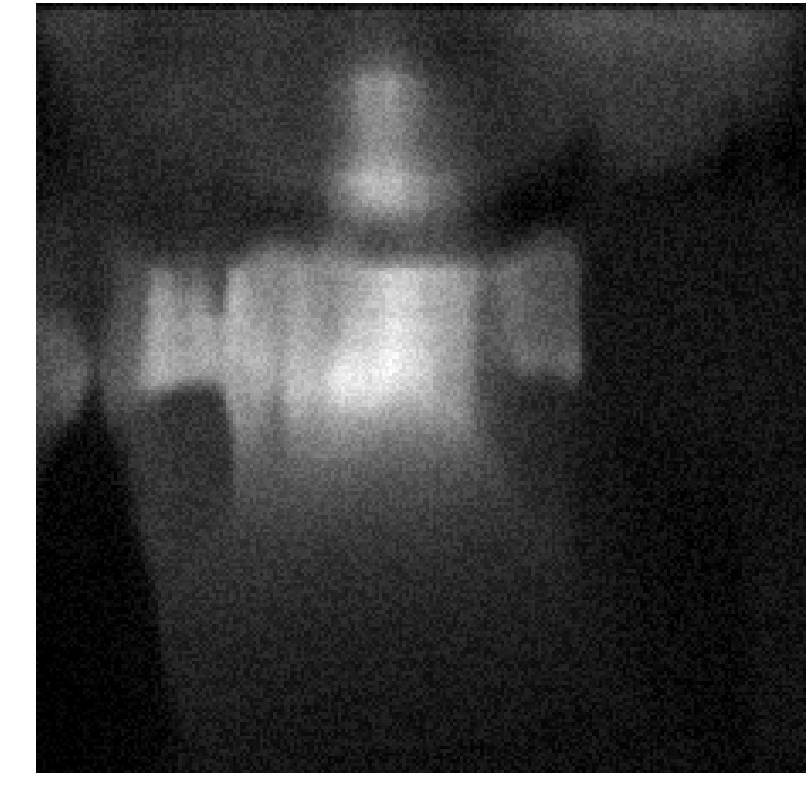
\includegraphics[width=0.32\textwidth]{images/depth_image3.png}}
\caption{Estimated order of a linear sequence of which the first 3 frames are shown in Figure \ref{fig:frames} with 99\% estimated probability for the correct order estimated by grayscale, 90\% for the correct order for the height above ground feature and 87\% for the wrong order estimated by the interpolated lidar, that incorrectly swaps the last two frames highlighted with a red border}
\label{fig:orderings}
\end{figure}

\section{Combining features}
Besides viewing the features as single information source, it is hypothesized that the lidar provides additional information to enrich the representation learned from camera alone and combinations of the feature maps should show even stronger performs. To study this in more detail several networks have been implemented containing separate backbones for both the lidar and image data for the initial layers. These backbones combine at different depths of the network to a single backbone processing the rest of the convolutional layers as single features. The concatenation of neurons is always applied after the possible pooling, batch norm and ReLU steps at a particular level, precisely before the next convolutional layer begins.

Initial experiments were carried out on the OPN3 network with the unprocessed lidar and grayscale images to get an general understanding of merging on different depths - better combinations of features for acquiring maximum accuracy are investigated next. Table \ref{tab:merge_results} shows that merging after the first convolutional layer gives indeed an improvement, but the difference is very marginal with 0.4\% over using only grayscale, and this can definitely fall within the limit of uncertainty of the training. It can be concluded that on the OPN3 task the enriched data does not directly lead to improved performance. 

Further investigations were performed on the OPN4 network to find the strength of different feature combinations. The three strongest feature maps on OPN4 with grayscale images, lidar height and interpolated lidar depth were selected for the more detailed investigation (color was not selected although it being stronger than lidar height, because grayscale is already generated from the same data source). An example of the order estimated by those individual features given a forward sorted permutation is shown in Figure \ref{fig:orderings} (interestingly enough the generally strongest interpolated depth feature does incorrectly swap the last images). The combination of the selected features continues to show strong performance close to 60\% accuracy, but it is rather surprisingly not better than the individual interpolated lidar depth feature alone. From those results it appears that combining the features does not directly lead to improved performance. 

Looking at the influence of the merging depth, it becomes clear that merging after the second convolutional layer appears to work the best and further in the network tend to be weaker with merging after the fourth convolutional layer not leading to convergence at all. Late fusion has however earlier been found to perform better\cite{schlosser2016}, although significant cost is noted for the large increase in the number of parameters. It is hypothesized that the difficulty of the learning problem increases so substantially in this task, with more parameters added for the various input sources, that the lack of training data samples could be a reason that no improved performance is seen on this particular task. 
%[OPN4 is still missing...]
%Further investigations were performed on the OPN4 network to find the strength of different feature combinations. The combination of grayscale and lidar shows much stronger performance on the OPN4 network, with a difference of around 6\%, considerably higher than the improvement in the OPN3 network.

\begin{table}[]
\centering
\caption{Accuracy results on the trained networks (italic indicates non-converging)}
\label{tab:merge_results}
\begin{tabular}{|p{7.5cm}|p{2cm}|p{2cm}|}
\hline
\textbf{Input}                                                          & \textbf{Output network} & \textit{\textbf{Accuracy}} \\ \hline
grayscale and unprocessed lidar merged after first convolution          & OPN3                    & 82.8 \%                   \\ \hline
grayscale and unprocessed lidar merged after third convolution          & OPN3                    & 79.5 \%                   \\ \hline
grayscale and unprocessed lidar merged after fourth convolution         & OPN3                    & \textit{49.6} \%          \\ \hline
grayscale, interpolated lidar depth and lidar height merged after first convolution          & OPN4                    & 58.5 \%                   \\ \hline
grayscale, interpolated lidar depth and lidar height merged after second convolution         & OPN4                    & 59.2 \%                   \\ \hline
grayscale, interpolated lidar depth and lidar height merged after third convolution          & OPN4                    & 52.7 \%                   \\ \hline
grayscale, interpolated lidar depth and lidar height merged after fourth convolution         & OPN4                    & \textit{4.3} \%                   \\ \hline
\end{tabular}
\end{table}

\section{Additional experiments}
As earlier works~\cite{misra2016,lee2017} have used the Caffenet backbone, the networks considered here so far, are focused on this architecture as well. However several other networks have been reported with superior performance on object detection on the Imagenet dataset, notably the Resnet architecture\cite{he2016}. The Resnet architecture has versions with various depths with increasing strength on particular task if properly trained. Because the binary ordering task has simple output and to shorten the learning time it could be argued that Resnet-18 should be solid choice to start. Testing on the OPN3 datasets and keeping other parameters similar to earlier experiments results the network however fails to converge with an accuracy of 53.1\% only slightly better than random and far worse than the networks based on Caffenet. The exact reason for this behavior has not been found, but it can be concluded that the Resnet architecture does apparently not easily adapt to this problem.

In another experiment the influence of the constant timing offset between the different frames was investigated. Under the assumption of relative constant velocity the traveled distances between frame with the same time offset is frequently on a similar scale. To check the influence of this a more difficult task was run with the time delay of all training data changed from the fixed 4 or 5 frames, to a sampled one from 4 until 10 frames. The eventual network was evaluated on the same test set as all other OPN3 candidates. An accuracy of 79.7\% was reached, from which it is clear that the learning does indeed exploits the constant offsets, but the impact of this effect appears to be limited as the task is supposed to be more difficult. The same experiment was carried out on the OPN4 network resulting in an accuracy of 37.3\% using only grayscale (instead of 51.2\% using the standard network). The difference is more apparent in this instance, but the network still achieves good performance. It is difficult to determine the exact influence of the constant offsets on the degraded performance as the task is also expected to be more difficult. 

Another experiment to investigate the focus of the network on particular environments was performed by checking if the network would only perform well on straight roads. Because the network is run on the visual odometry dataset, the GPS data could be used to extract the heading to determine if the vehicle is turning. Unfortunately this data was only available for the original training dataset, which consisted of the initial 11 sequences. These sequences were however included in the generated training set in all earlier experiments. For this experiment a new training set was therefore generated from the 11 until the 21 sequence (the original test data) and for the new test dataset frames with turns were sampled from sequence 0 to 10 using the odometry information. Interestingly the network reached still a performance of 57.2\% on only corners compared to 61.6\% over the whole dataset using only the grayscale images (note that either the last 10 sequences are better for training or the first 10 sequences are generally easier to sort for the network as the percentage on the default task is already significantly higher). The network apparently performs strong on corners as well, while these are far less common in the training dataset. 

% In general all the networks that converge exhibit significant over-fitting, with accuracies reaching close to 100\% on the training data with the L2 regularization employed. As accuracy percentages are also high on the test task it is clear that the task is relatively easy for the neural network to learn, as was noticed earlier by Fernando et al.~\cite{fernando2017}. Therefore all succesful experiments on the OPN3 have also been carried out on the full OPN network\cite{lee2017}, with 4 images as input and permutation labeling. In contrast to the OPN4 network which does not distinguish between forward and backward orderings of the same permutation, in this work the network are trained with all permutation labels differently as in driving the difference between going forward (as would happen in reality) and going backward should generally be detectable. 

% grayscale with training on non-fixed time differences                   & Caffenet                  & OPN3                    & 79.72 \%                   \\ \hline
% grayscale                                                               & Resnet-18                 & OPN3                    & \textit{53.12} \%          \\ \hline
% grayscale                                                               & Caffenet                  & OPN4                    & 38.63 \%                   \\ \hline
% grayscale and unprocessed lidar merged after first convolution          & Caffenet                  & OPN4                    & 44.42 \%                   \\ \hline

%In an initial experiment, we implement the tuple network from\cite{misra2016}. [However it did not converge].

%Describe the evaluation you did in a way, such that an independent researcher can repeat it. Cover the following questions:
% \begin{itemize}
%  \item \textit{What is the experimental setup and methodology?} Describe the setting of the experiments and give all the parameters in detail which you have used. Give a detailed account of how the experiment was conducted.
%  \item \textit{What are your results?} In this section, a \emph{clear description} of the results is given. If you produced lots of data, include only representative data here and put all results into the appendix. 
% \end{itemize}
